\documentclass[12pt]{article}
\usepackage{float}
\usepackage{caption, subcaption}
\usepackage[T1]{fontenc}
\usepackage[backend=bibtex, maxbibnames=99, sorting=none]{biblatex}
\addbibresource{sample.bib}
\usepackage{url}
\usepackage[utf8]{inputenc}
\usepackage{amsmath}
\usepackage{setspace}
\usepackage{graphicx}
\graphicspath{{Images/}}
\usepackage{parskip}
\usepackage{multirow}
\usepackage{enumitem}
\usepackage{amssymb}
\usepackage{framed}
\usepackage{fancyhdr}
\usepackage{vmargin}
\usepackage{subcaption} %usamos subcaption mejor que subfig (más moderno)
\usepackage{eurosym}
\usepackage[table,xcdraw]{xcolor} % add color to your tables
\usepackage[bottom]{footmisc} %footnotes
\definecolor{blau}{RGB}{210,235,255}
\definecolor{blau2}{RGB}{120,170,225}
\setmarginsrb{2.5 cm}{2 cm}{2 cm}{2.5 cm}{1 cm}{0.5 cm}{1 cm}{1 cm}

\usepackage{multirow}

\usepackage{chngcntr}

\usepackage[framed, numbered]{matlab-prettifier}
 
\counterwithin{figure}{section}
\counterwithin{table}{section}
\numberwithin{equation}{section}

\usepackage{titlesec}
\usepackage{hyperref}
\usepackage{listings}
\usepackage{multicol}
\setlength{\columnsep}{1cm}

\titleclass{\subsubsubsection}{straight}[\subsection]

\newcounter{subsubsubsection}[subsubsection]
\renewcommand\thesubsubsubsection{\thesubsubsection.\arabic{subsubsubsection}}
\renewcommand\theparagraph{\thesubsubsubsection.\arabic{paragraph}} % optional; useful if paragraphs are to be numbered

\titleformat{\subsubsubsection}
  {\normalfont\normalsize\bfseries}{\thesubsubsubsection}{1em}{}
\titlespacing*{\subsubsubsection}
{0pt}{3.25ex plus 1ex minus .2ex}{1.5ex plus .2ex}

\makeatletter
\renewcommand\paragraph{\@startsection{paragraph}{5}{\z@}%
  {3.25ex \@plus1ex \@minus.2ex}%
  {-1em}%
  {\normalfont\normalsize\bfseries}}
\renewcommand\subparagraph{\@startsection{subparagraph}{6}{\parindent}%
  {3.25ex \@plus1ex \@minus .2ex}%
  {-1em}%
  {\normalfont\normalsize\bfseries}}
\def\toclevel@subsubsubsection{4}
\def\toclevel@paragraph{5}
\def\toclevel@paragraph{6}
\def\l@subsubsubsection{\@dottedtocline{4}{7em}{4em}}
\def\l@paragraph{\@dottedtocline{5}{10em}{5em}}
\def\l@subparagraph{\@dottedtocline{6}{14em}{6em}}
\makeatother

\usepackage[table,xcdraw]{xcolor}

\setcounter{secnumdepth}{4}
\setcounter{tocdepth}{4}


\usepackage{pdflscape} %Per poder posar la pàgina en horizontal
\usepackage{multicol} %Escriure en columnes 
 
	% Author
\date{\today}							% Date

\makeatletter
\let\thetitle\@title
\let\theauthor\@author
\let\thedate\@date
\makeatother

\pagestyle{fancy}
\fancyhf{}
\lhead{21D009 Networks: Concepts and Algorithms}
\rhead{Movie recommendations using networks}
\cfoot{\thepage}

\begin{document}

\begin{titlepage}
	\centering
    
\includegraphics[scale = 0.7]{bse_logo.png}\\[1.2 cm]	% University Logo
    \textsc{\LARGE Barcelona School of Economics}\\[2.0 cm]	% University Name
	\textsc{\Large Data Science Methodology Program}\\[0.5 cm]				% Course Code
	\textsc{\large 21D009 Networks: Concepts and Algorithms }\\[0.5 cm]				% Course Name
	\rule{\linewidth}{0.2 mm} \\[0.4 cm]
	{ \huge \bfseries Movie recommendations using networks }\\
	\rule{ \linewidth}{0.2 mm} \\[1.5 cm]
	
\begin{center}
    
{ \emph{Authors: }\\
    \textsc{Codd}, Jonny \\
    \textsc{Chen}, Joshua \\
    \textsc{Gallegos}, Rafael \\
    \textsc{Pérez}, Carlos \\ } 

\vspace{0.7cm}


    \textit{Professors:}\\  \textsc{Milán}, Pau \\
    	\textsc{Komander}, Björn
        \\ \vspace{0.5cm}


\vspace{1.7cm}


{\large December $20^{th}$, 2023} \\[2 cm]

 \end{center}
	\vfill
	
\end{titlepage}
	
\tableofcontents
\vspace{1cm}
\listoffigures
\listoftables
\pagebreak

\newpage

\section{Introduction}

Popular recommendation techniques in Machine Learning often apply many network and network-adjacent concepts to create personalized recommendations. The matrix of user-to-item scores can be thought of as the adjacency matrix of a bipartite network - with the users representing one set of nodes and the items representing the other. The edges are represented either by binary or scalar relationships between users and items, implying unweighted or weighted graphs respectively.

Our project is two-fold. Using the concepts learned in this course, we will first analyze one of these networks to identify trends and patterns and extract information. We will then study and build recommendation systems and propose/implement new strategies and techniques derived from the first part to improve methodologies.

\section{Literature Review}

\section{Dataset}

MovieLens is popular movie recommender system dataset developed by GroupLens, a computer science research lab at the University of Minnesota. The goal of this challenge is to recommend movies to its users based on their movie ratings. Group Lens offers datasets of different sizes and their datasets are widely used in research and teaching contexts.

The selected dataset consists mainly on two files: movies.csv and ratings.csv. Movies dataset has 9,742 unique films and a column indicating the genres of the film. All possible genres are: 'Romance', 'Musical', 'Children', 'Documentary', 'Sci-Fi', 'Film-Noir', '(no genres listed)', 'Crime', 'Mystery', 'Drama', 'Western', 'Fantasy', 'Animation', 'Thriller', 'War', 'Action', 'Adventure', 'IMAX', 'Comedy', 'Horror'. The number of movies per genre is represented in Figure \ref{fig:count_genre}.

Ratings dataset consists of 100,836 ratings with 610 unique users that rated 9,724 movies. As it can be observed in Figure \ref{fig:count_rating}, the ratings from users are right-skewed, which suggests that users tend to enter their rating on movies that they probably have liked. Ratings from users have been registered from 1996-03-29 until 2018-09-24. The most popular movies among users have been: Shawshank Redemption, The (1994), Godfather, The (1972), Fight Club (1999), Godfather: Part II, The (1974) and Goodfellas (1990).

\begin{figure}[h!]
    \begin{minipage}[b]{0.49\linewidth}
         \centering
  	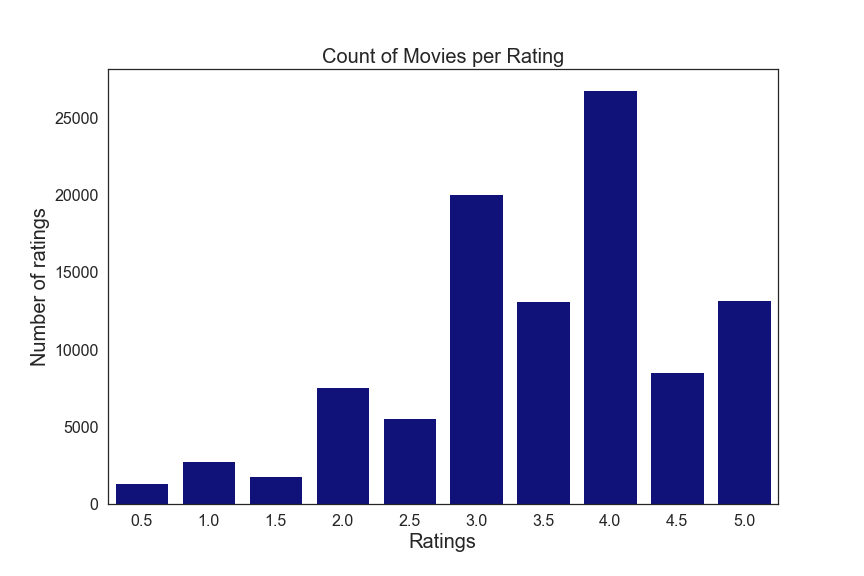
\includegraphics[width=0.99\textwidth]{count_rating.png}
  	\caption{Count of Movies per Rating}
  	\label{fig:count_ranking}
    \end{minipage}
    \hspace{0.01cm}
    \begin{minipage}[b]{0.49\linewidth}
        \centering
  	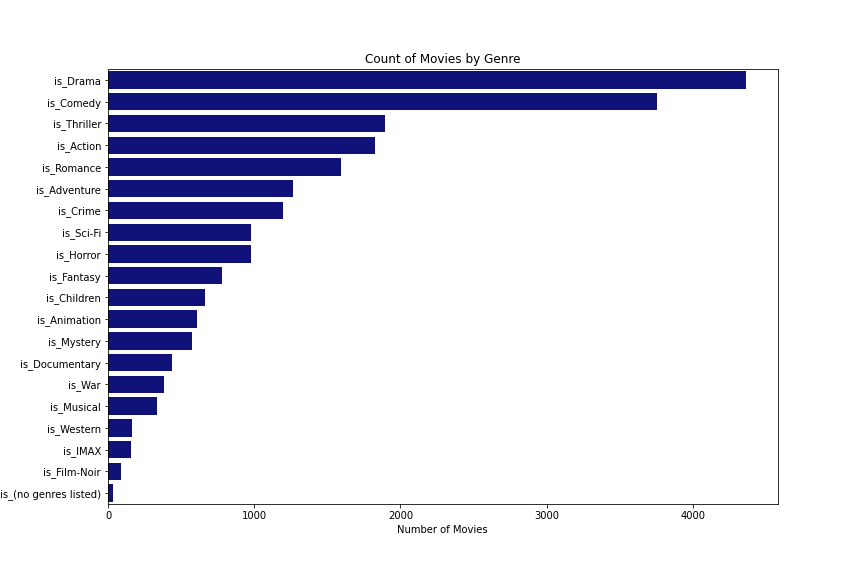
\includegraphics[width=0.99\textwidth]{count_genre.png}
  	\caption{Count of Movies per Genre}
  	\label{fig:count_genre}
    \end{minipage}
\end{figure}

The median user has rated 70 films, whereas the user with the lowest number of watched films was 20 movies and the user with the highest number of rated films is 2698.

\begin{figure}[h!]
    \begin{minipage}[b]{0.49\linewidth}
         \centering
  	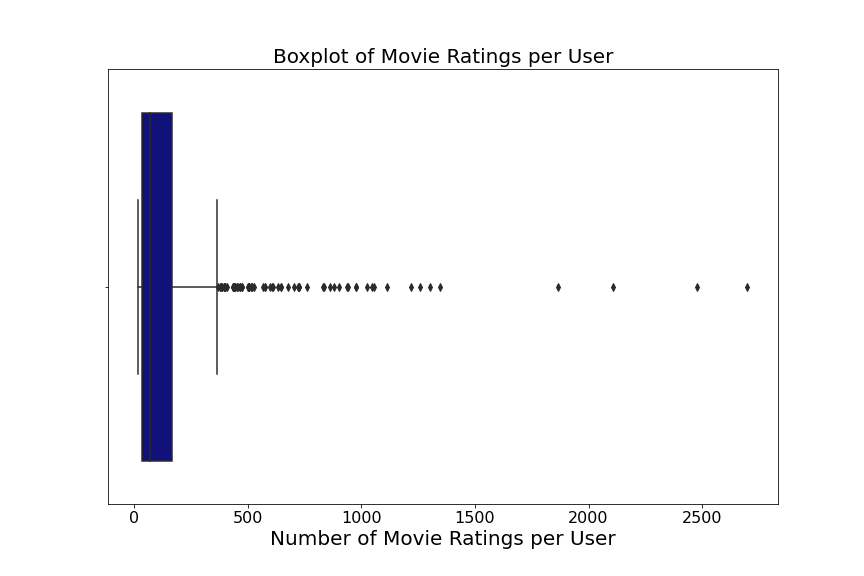
\includegraphics[width=0.99\textwidth]{count_user.png}
  	\caption{Count of Movies per User}
  	\label{fig:count_user}
    \end{minipage}
    \hspace{0.01cm}
    \begin{minipage}[b]{0.49\linewidth}
        \centering
  	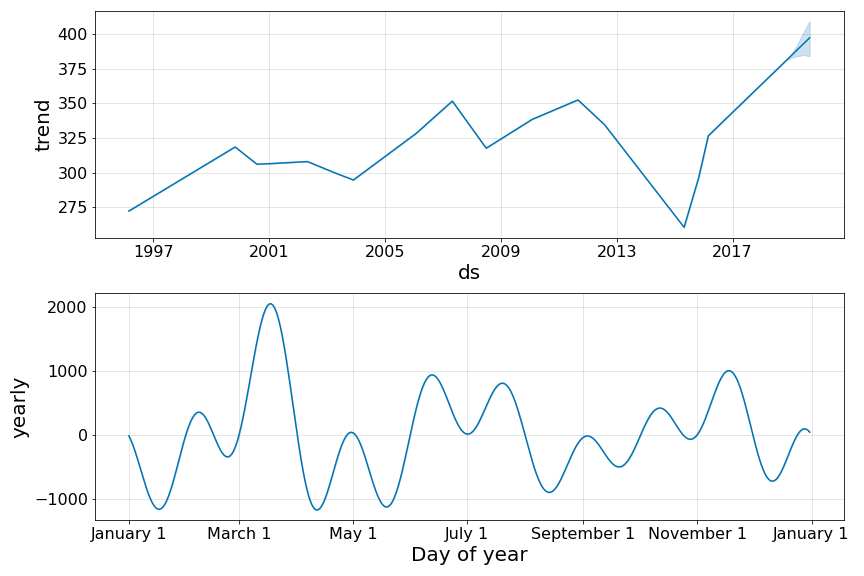
\includegraphics[width=0.99\textwidth]{prophet.png}
  	\caption{Time Series Analysis of Ratings with Prophet}
  	\label{fig:ranking_ts}
    \end{minipage}
\end{figure}

\section{Network analysis}

With the MovieLens dataset, we created 4 different networks.  The first, the user-movie network, is the aforementioned user-item network that will serve as the foundation for both the other networks and the recommendation systems that we build. From this network, we also
constructed a user-to-user network - a symmetric unipartite network capturing the similarity between users. Similarly, we did this for the movies as well. Finally, we created another bipartite network that, instead of capturing relationships between users and specific movies, it describes the "fan score" between a user and a genre of movie.

\subsection{User and movie bipartite network}

Despite an incredibly sparse matrix, understandably with close to 10,000 movies - this results in a connected graph - meaning there is only one component.

To better understand that users and movies, we calculated the centrality for each of them:
With this graph - the degree centrality for users and movies are aligned with how many reviews they have. The centrality score for users is much higher than that for movies as there are many more reviews per user than there are per movie.

However, this may not be the best way to actually capture centrality as highly central movies and users might not just be how many direct nodes that they have. Therefore, we also calculated the betweenness and closeness centralities

\begin{figure}[H]
\centering
\caption{Network Centrality Measures and Comparative Metrics for Movies}
    \begin{tabular}{|c|c|c|c|}
        \hline
        \textbf{User Id} & \textbf{Degree Centrality} & \textbf{Betweeness Centrality} & \textbf{Closeness Centrality} \\ 
        \hline
        599 & 4.067 & 0.141 (1) & 0.406 (2) \\
        414 & 4.429 & 0.131 (2) & 0.413 (1) \\
        474 & 3.460 & 0.120 (3) & 0.395 (3) \\
        448 & 3.061 & 0.110 (4) & 0.388 (4) \\
        274 & 2.210 & - & 0.373 (5) \\
        610 & 2.136 & 0.060 (5) & 0.372 (6) \\
        68  & 2.067 & - & 0.371 (7) \\
        380 & 2.000 & 0.034 (10) & 0.370 (8) \\
        606 & 1.829 & 0.050 (6) & 0.367 (9) \\
        288 & 1.731 & - & 0.365 (10) \\
        \hline
    \end{tabular}

   \vspace{0.2cm} % Adjust the vertical space between tables as needed
    
    \begin{tabular}{|p{6cm}|r|r|r|}
        \hline
        \textbf{Movie Title} & \multicolumn{1}{p{2.5cm}|}{\textbf{Degree Centrality}} & \multicolumn{1}{p{3cm}|}{\textbf{Betweeness Centrality}} & \multicolumn{1}{p{3cm}|}{\textbf{Closeness Centrality}} \\
        \hline
        Forrest Gump (1994) & 0.0339 & 0.0064 & 0.4824 \\
        Pulp Fiction (1994) & 0.0316 & 0.0050 & 0.4650 \\
        Matrix, The (1999) & 0.0286 & 0.0048 & 0.4694 \\
        The Silence of the Lambs (1991) & 0.0287 & 0.0046 & 0.4624 \\
        Shawshank Redemption (1994) & 0.0326 & 0.0042 & - \\
        Star Wars: Episode IV (1977) & 0.0258 & 0.0041 & 0.4613 \\
        Jurassic Park (1993) & 0.0245 & - & - \\
        Braveheart (1995) & 0.0244 & - & - \\
        Terminator 2 (1991) & 0.0231 & - & - \\
        Schindler's List (1993) & 0.0226 & - & - \\
        \hline
    \end{tabular}
\end{figure}
\subsection{User-to-user network}

The user-to-user network is calculated by 

\subsection{Movie-to-Movie network}

\subsection{User-to-Genre network}

\section{Collaborative Filtering}

\section{Graphical Neural Networks}

\newpage
\section{Conclusions}
\vspace{1em} 


%\bibliographystyle{plain}
%\bibliography{Bibliography.bib}

\newpage
\printbibliography[heading=bibintoc]

\end{document}